\documentclass[hidelinks]{article}

\usepackage{fullpage} % Package to use full page
\usepackage{parskip} % Package to tweak paragraph skipping
\usepackage{tikz} % Package for drawing
\usepackage{amsmath}
\usepackage{hyperref}
\usepackage{enumitem}
\usepackage{float}
\usepackage{ upgreek }
\usepackage[explicit]{titlesec}
\usepackage{graphicx}
\usepackage {verbatim}
\newcommand{\RNum}[1]{\uppercase\expandafter{\romannumeral #1\relax}}
%\titleformat{\section}{\normalfont\Large\bfseries}{}{0em}{#1\ \thesection}

\title{Inlämning 2 \\ Objektorienterad programmering med Java}
\author{Emil Björklund - embj3739 \\ emilbjorklund@live.com}


\begin{document}

\maketitle 
\newpage

\section*{Inledning}
\begin {itemize}
\item IDE: Eclipse IDE v4.5.0
\item Java verision: JDK 8 update 191
\item OS: MacOS Mojave
\end{itemize}

\textbf{Note.} Källkoden bifogas i separat .zip som finns i inlämningen. Det finns ett packet som har alla classer. Classen game är den som skall anropas.

\section*{Struktur - UML}
\begin{figure}[H]
\centering
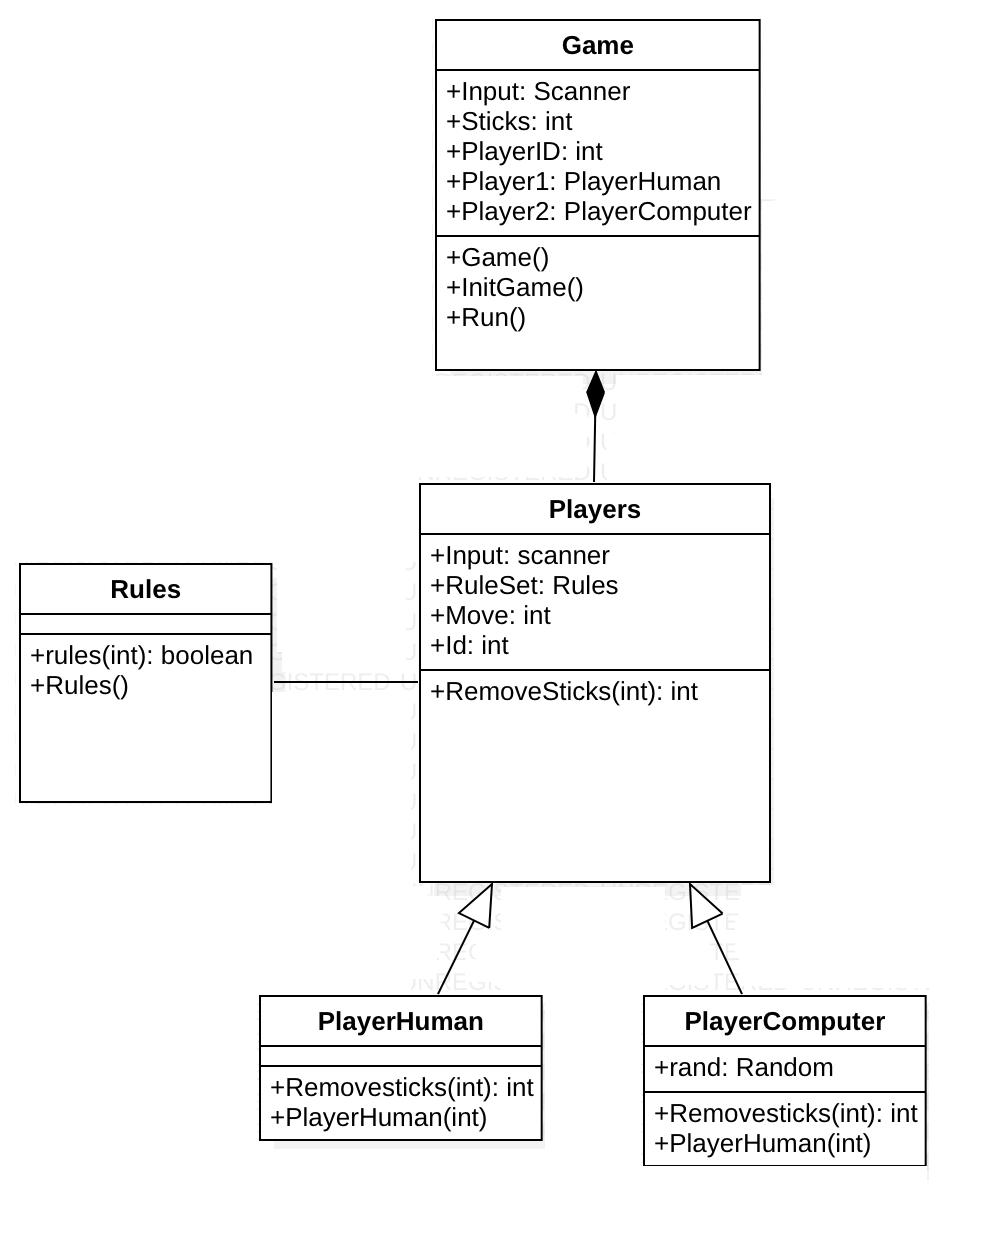
\includegraphics[scale=0.30]{pic}
\caption{UML}
\end{figure}
\newpage

\section*{Upplägg}
Programmet består av 5 klasser som alla har sin roll. Programmet är designat att fungera för olika typer av spel där människa kan möta människa eller människa möter dator. Datorn kan även spela mot sig själv.
För att ändra spelupplägg deklarerar man bara olika objekt för människa kontra dator.
Klassen game är programmets huvudklass och innehåller main funktionen där objektet game deklareras.

För att skydda input från konsolen så används metoden hasNextInt för att säkerställa att endast integers tas emot i programmet.
\begin{verbatim}
while (!input.hasNextInt()) input.next();
\end{verbatim}

Klassen PlayerComputer använder sig av rand för att slumpvis välja ett drag som är tillåtet inom spelets regler. Eftersom Random från java.util är en “blackbox” så används try och catch för att skydda operationen som hämtar en slumpad integer.
Spelets regler implementeras I en separat class för att skilja dom åt från funktionaliteten hos spel klasserna.

\subsection*{Metoder}
\textbf{initGame()} - Printar till konsollen och tar emot input för hur många sticks som skall användas. Slutligen anropas run().\\ \\
\textbf{run()} - Metoden run() loopas med en while tills att det är gameover. Ifsatser som är beroende av turn variablen anropar objekten player 1 och player2. Objeketen retunerar hur många sticks som är kvar. Om det är en stick kvar kommer en annan sats bli sann och avsluta spelet. \\ \\
\textbf{removeSticks()} - Denna metod tar bort sticks. Om det är human som använder metoden så skickas draget till roules för att kolla om draget är lagligt. Om computer använder metoden anropas rand för att generera ett drag. \\ \\
\textbf{rules()} - ruels() tar in en integer och kollar om draget är möjligt beroende på reglerna. Metoden retunerar true eller false.








\end{document}